% do not change this formatting 
\documentclass[10pt]{article}
\parindent=0pt \parskip=8pt
\textwidth=3in
\hoffset=.3in 
\usepackage{amssymb,amsmath,amsthm,mathrsfs} 
\pagestyle{headings}
\usepackage{amsmath}
\newcommand*{\QEDA}{\hfill\ensuremath{\blacksquare}}%
\usepackage[margin=1in]{geometry}
\usepackage{xcolor}
\usepackage{amsthm}
\usepackage{url}
\usepackage{shadethm}
\usepackage{mathtools}
\usepackage{systeme}
\usepackage{float}
\usepackage{mathtools}
\setlength\parindent{24pt}
\newcommand\numberthis{\addtocounter{equation}{1}\tag{\theequation}}
\usepackage{caption}
\usepackage{subcaption}
\newtheorem{theorem}{Theorem}
\usepackage{dcolumn}
\newcolumntype{2}{D{.}{}{2.0}}
\usepackage{subfig}
\usepackage{mwe}


\usepackage[utf8]{inputenc}


\newshadetheorem{thm}{Theorem}
\definecolor{shadethmcolor}{HTML}{EDF8FF}
\definecolor{shaderulecolor}{HTML}{45CFFF}
\setlength{\shadeboxrule}{.4pt}

% replace 'n' with the number of the homework assignment
\title{Analyzing Biological Models with the Wasserstein Distance}

% replace 'your name here' with your name
\author{
  Shane Lubold\\
  \texttt{shane.lubold@asu.edu}\\
  Arizona State University
  \and
  Sebastien Motsch \\
  \texttt{smotsch@asu.edu}\\
  Arizona State University
}
\date{\today}

\begin{document}
\maketitle


\begin{abstract}
In recent years a number of mathematical models have been proposed that describe biological systems. One needs a way to compare the accuracy of these methods, in relation to each other and in relation to empirical data. The Wasserstein distance is a new metric that can be used for such a purpose. In one dimension, there exists a closed form expression for the Wasserstein distance, but in two or more dimensions, no such expression exists for most functions. In this paper we present a method for approximating the Wasserstein distance in two or more dimensions. We also consider several biological models and demonstrate how the Wasserstein distance can be used to analyze the effictiveness of such models.
\end{abstract}


\begin{center}
\textbf{Recent progress:}
\end{center}

\begin{enumerate}
\item Went through the 1D,2D non-bio work. All data files for images in 1D section have been saved to folder ``Data for Paper''. Also fixed wording in section. 
\item For 1D bio work, saved data in folder ``Data for Paper''
\begin{itemize}
\item Put in images of rhoMicro, rhoMacro at time initial and final. 
\item Fitted WD to N, Log(WD) to Log(N) and fitted WD to $\Delta x$, saved data.
\item Computed rhoMicro, rhoMacro velocity, included images, saved data.
\end{itemize}
\item For 2D bio work, 
\begin{itemize}
\item Put in some basic wording
\item Wrote Velocity code, included Macro velocity image and data in folder. 
\item Fixed micro code.
\item Added WD code for 2D (took old simplex method code and call it in 2DStochasticFinal).
\end{itemize}
\textbf{Questions:} 
\begin{itemize}
\item Normalization of Micro
\item How large are our systems for the 2D bio? Even 121 variables takes 4.5 minutes to compute. Might try hungarian algorithm, interior point methods, etc to speed up.
\end{itemize}
\end{enumerate}

\newpage
\section{Introduction}

  Modeling biological systems has increased in popularity in recent years. From bacteria to swarm bees, a number of models have been proposed to describe each system. But the increase in number of models does not necessary improve the comprehension of the underlying population. One needs to be able to compare there predictions and more important to measure their agreement with experimental data. One way to do this is to use the Wassertstein distance, which allows us to compare discrete and continuous dynamics (i.e.e, systems of ODEs and PDEs). But so far Wasserstein distance has been used mainly as a powerful tool to prove analytic results (i.e. existence/uniqueness of solutions). In this paper we use the Wasserstein distance to compare the accuracy of biological models in relation to empirical data. 


The challenge is that the Wasserstein distance, defined as a minimization problem,
can only be computed explicity in one dimension. In two or higher dimensions, we must rely on an approximation. In this paper, we develop a numerical method that approximates the Wasserstein distance through the Simplex method for continuous distributions, and the Hungarian algorithm for discrete distributions (sets of points). Once the numerical methods have been implemented and tested, we will use the Wasserstein distance to perform data-model comparison for several dynamics (e.g. pedestrian dynamics, swarming model). In many studies, data-model comparisons are limited to only visual or qualitative agreement. This framework aims at providing quantitative measurement for the agreement (or discrepancy) between a model and experimental data.

The rest of the paper is organized as follows. In Section \ref{sec: Preliminaries}, we present the general problem, outline the theory and notation, and provide some theoretical results regarding the Wasserstein Distance. In Section \ref{sec: OneD}, we provide the theory and computations of the Wasserstein distance in one dimension. We also consider the case of noisy data and show how this affects the computation of the Wasserstein distance. Section \ref{sec: TwoD} outlines the problem in two dimensions, and shows how the simplex method may be used to compute the Wasserstein distance between continuous and discrete distributions. In Section \ref{sec: BioSystems} we examine how models used to study biological systems compare to empirical data through the use of the Wasserstein distance. Section \ref{sec: Conclusion} provides concluding remarks and points to future work.


\section{Literature Review} 
The optimal transport problem, the problem of moving a mass from one location to another in the most efficient way possible, has been studied for several centuries. One way to phrase the problem is this. Consider a number $n$ of bakeries, each of which makes a certain amount of bread, and we know that there are $m$ restaurants that will consume a fixed amount of bread. Since the amount of bread produced and consumed is fixed for each bakery and restaurant, we can model these quantities as probability measures and create a ``density of production" and a ``density of consumption" on some space, which we can consider to be a metric space with the distance between a bakery and a restaurant as the length of the straight line between them. The optimal transport problem then seeks to move the bread from the bakeries to the restaurants by minimizing the total cost of transportation. For a more complete description of this problem, see Section 3 of \cite{CVillani}.

\noindent Recent work has shown a number of theoretical properties of the Wasserstein distance, including the existence of solutions to the optimal transport problem under certain assumptions, \cite{CVillani}, the convexity of the solution space, \cite{AN}, and the weak convergence of measures, \cite{AN}. 

\noindent In recent years there has been a proliferation of biological models concerning a vast array of biological systems. 

\section{Preliminaries}
\label{sec: Preliminaries}
Given a Polish (complete, separable, metric) space $(M,d)$, define $\mathcal{P}(M)$ as the set of probability measures on $(M, \mathcal{B}(M))$. If $X, Y$ are two Polish spaces, $T$ is a Borel map, and $\phi \in \mathcal{P}(X)$ is a measure, we can define $T_{\#}\phi \in \mathcal{P}(Y)$, which we call the \textit{pushforward of $\phi$ through T}, as 
\begin{equation}
T_{\#}\phi(A) = \phi(T^{-1}(A)), \ \ \ \ \ \forall A \subseteq Y, \  A \  \text{is Borel}.
\label{eq: TransportDefn}
\end{equation}
The pushforward of $\phi$ through $T$ has the property that
\begin{equation}
\int_Y h \ dT_{\#}u = \int_X h \circ T d\mu,
\label{eq: TransportProperty}
\end{equation}
for every Borel function $h: Y \rightarrow \mathbb{R} \cup \{\pm \infty\}$. Define a Borel cost function $c: X \times Y \rightarrow \mathbb{R} \cup \{\infty\}$. Following the notation of \cite{AN}, we call the following problem formulation the \textit{Monge optimal transport problem}.

\noindent \textbf{Monge Optimal Transport Problem:} Let $v \in \mathcal{P}(X)$, $\mu \in \mathcal{P}(Y).$ We define the $j$th Wasserstein distance between $v$ and $\mu$ as
\begin{equation}
W_j(\mu,\nu) = \inf_{T} \sqrt[\leftroot{-2}\uproot{2}j]{\int_{M}c(x, T(x))^{j} \ d\mu(x)},
\label{eq: CostWassDist}
\end{equation}
where the $\inf$ is taken over all $T$ satisfying (\ref{eq: TransportProperty}). As noted in \cite{AN}, Monge's definition can be ill-posed if no such admissible T exists (if $\mu$ is a Dirac delta and $\nu$ is not) or if the constraint that $T_{\#}\mu = \nu$ is not weakly sequentially closed, w.r.t any reasonable weak topology. To resolve these issues, we also present the formulation attributed to Kantorovich, \cite{AN}.

\noindent \textbf{Kantorovich Optimal Transport Problem:}
\noindent For each $\mu \in \mathcal{P}(X)$ and $\nu \in \mathcal{P}(Y)$, let $\Pi(f,g)$ denote the collection of couplings between $\mu$ and $\nu$. In other words, 
\begin{equation}
\Pi(f, g) = \Big\{\pi: \pi(A \times M) = \mu(A), \ \text{and} \ \pi(A \times M) = \nu(A), \ \text{for each $A \in \mathcal{B}(M)$}  \Big\}.
\label{eq: Couplings}
\end{equation}
We then define the $j$-th Wasserstein distance between $\mu$ and $\nu$ as 
\begin{equation}
W_j(f, g) = \inf_{\pi \in \Pi(f, g)}\sqrt[\leftroot{-2}\uproot{2}j]{\int_{M \times M} d(x,y)^{j} d\pi(x, y)},
\label{eq: CouplingsWassDist}
\end{equation}
where the $\inf$ is taken over all $\pi \in \Pi(f, g)$ that satisfy (\ref{eq: Couplings}). In some cases, $W_p(\mu, \nu) = \infty$, so we will restrict ourselves $W_j(f, g)$ to $\mathcal{P}_j(M) \subset \mathcal{P}(M)$, where $\mathcal{P}_j(M)$ denotes the set of probability measures on M with finite $j$-th moment. In other words, 
\begin{equation}
\mathcal{P}_j(M) = \Big\{f \in \mathcal{P}(M): \int_M d(x, y)^j f(dy) < \infty, \ \text{for some $x \in M$} \Big\}.
\label{eq: jPM}
\end{equation}
As shown in \cite{AN}, $\Pi(f, g)$ is a convex set that contains $f \times g$.  If $c$ is lower semicontinuous and bounded below, then there exists a $\pi \in \Pi(f, g)$ that satisfies (\ref{eq: CouplingsWassDist}). \cite{AN} also proves that if $c$ is continuous and $\mu$ is non atomic, then the values of (\ref{eq: CostWassDist}) and (\ref{eq: CouplingsWassDist}) are equal.
It is also possible to show that $W_{j}$ defines a distance function on $\mathcal{P}_j(M)$. Clearly $W_{j}(\mu, \nu) = W_{j}(\nu, \mu)$ and $W_{j}(\nu, \mu) \geq 0$, with equality only holding in the case that $\mu = \nu$. To prove that $W_{j}(\mu, \nu) \leq W_{j}(\nu, \psi) + W_{j}(\psi, \nu)$ for some measure $\psi$, it's convenient to use the so-called gluing lemma, \cite{CVillani}.

\noindent \textbf{Gluing Lemma:} Let $(X_i, \mu_i), i = 1, 2, 3,$ be Polish probability spaces. If $(X_1, X_2)$ is a coupling of $(\mu_1, \mu_2)$ and $(Y_2, Y_3) $ is a coupling of $(\mu_2, \mu_3)$, then it is possible to construct a triple of random variables $(Z_1, Z_2, Z_3)$ such that $(Z_1, Z_2)$ has the same law as $(X_1, X_2)$ and $(Z_2, Z_3)$ has the same law as $(Y_2, Y_3)$.

\noindent For the remainder of the paper, we restict ourselves to $(M,d) = (\mathbb{R}^n, d)$, with $n \geq 1$ and $d$ being the standard metric on $\mathbb{R}^n$. 

\section{One Dimensional Case} \label{sec: OneD}
In one dimension, there exists a closed form solution to computing the Wasserstein distance between two probability density functions. Let $f, g: \mathbb{R} \rightarrow \mathbb{R}$ be functions such that
\begin{equation}
\int_{\mathbb{R}} f(x) \ dx = \int_{\mathbb{R}} g(x) \ dx.
\end{equation}
If we define
\begin{equation}
F(x) = \int_{- \infty}^x f(s) \ ds \ \ \ \ \text{and} \ \ \ \ G(x) = \int_{- \infty}^x g(s) \ ds,
\end{equation}
then the $2$nd Wasserstein distance between $f$ and $g$ is
\begin{equation}
W_2^2(f, g) = {\int_{0}^1 |F^{-1}(y) - G^{-1}(y)|^2 \ dy}.
\label{eq: 1DWD}
\end{equation}
From now on, we will refer to the value of ($\ref{eq: 1DWD}$) as the Wasserstein distance between $f$ and $g$, or simply the WD between $f$ and $g$.
One can think of (\ref{eq: 1DWD}) as moving the $j$-th percentile of $f$ to the $j$-th percentile of $g$ (Figure \ref{fig: 1DWD}).

\begin{figure}[H]
\centering
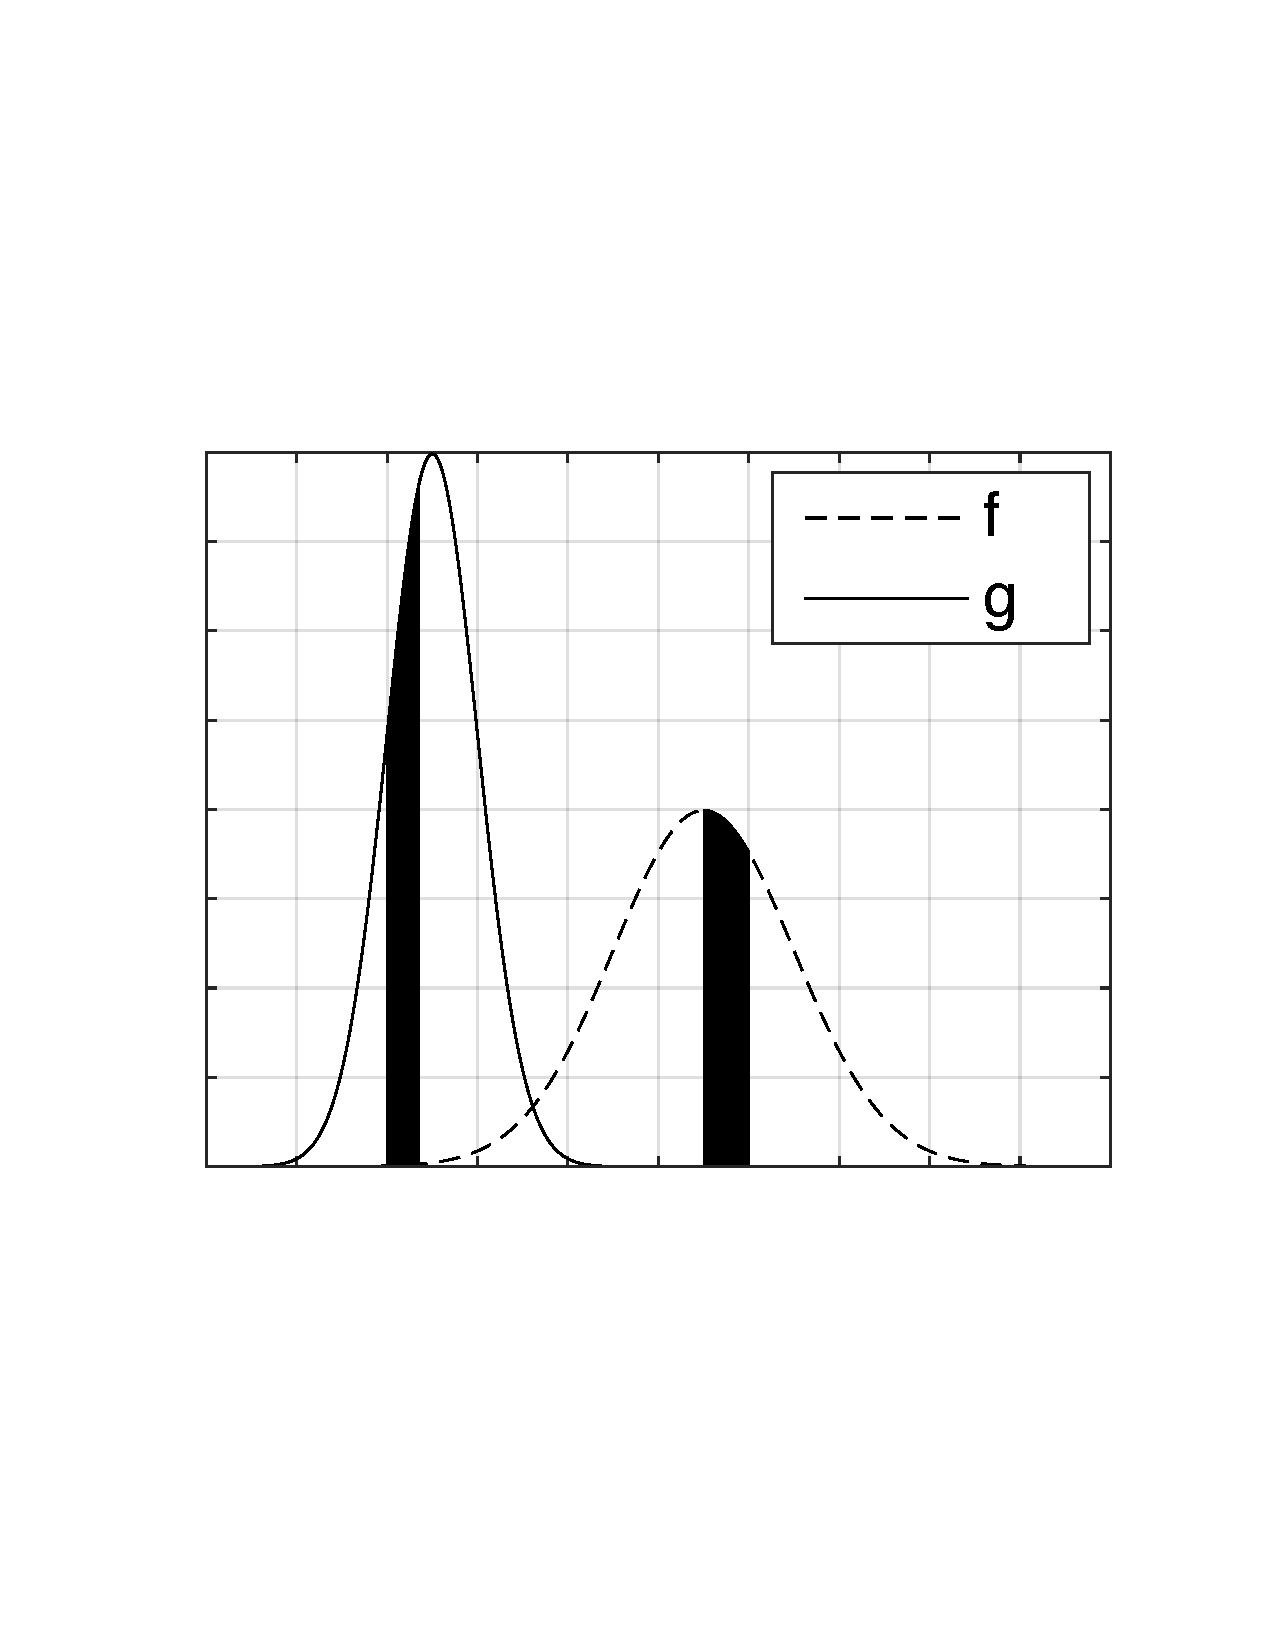
\includegraphics[scale = .4]{2ndPPercentile.pdf}
\caption{Moving $j$-th percentile (shaded) of $f$ to $j$-th percentile of $g$.}
\label{fig: 1DWD}
\end{figure}
%In some cases, it is possible the data one collects are corrupted by noise, and a relavent question is what are the mean and variance of the resulting approximation of the Wasserstein distance. Assume we observe $\textbf{f}$, $\textbf{g}$\footnote{From here on, boldface variables denote random variables.}, and we want to know the expected value and variance of our estimates of $W_1(f,g)$.
%\begin{equation}
%\textbf{f}(x) = f(x) + v, \ \ \ \textbf{g}(x) = g(x) + v, \ \ \ \ v \sim \mathcal{N}(0, \rho^2).
%\end{equation}
%When $j = 1$, (\ref{eq: Alt1DWD}) becomes
%\begin{equation}
%W_1(f, g) = \int_{-\infty}^\infty |f(x) - g(x)| \ dx.
%\end{equation}
%By linearity, we have that
%\begin{align*}
%\mathbb{E}(W_1(\tilde{f}, \tilde{g})) &= \mathbb{E}\Big(\int_{-\infty}^\infty |\textbf{f}(x) - \textbf{g}(x)| \ dx \Big) \\  & = 
%\int_{-\infty}^\infty |\mathbb{E}(\textbf{f}(x)) - \mathbb{E}(\textbf{g}(x))| \ dx \\
%&= \int_{-\infty}^\infty |f(x) - g(x)| \ dx = W_1(f,g) \numberthis \label{eq: MeanWD}
%\end{align*}
%From (\ref{eq: MeanWD}) we see that the addition of mean zero Gaussian noise does not on average affect our estimate of $W_1(\textbf{f}, \textbf{g})$. It is not possible to show, however, the same result when $ j \geq 2$, since for a non-linear function $g$, $\mathbb{E}(g(x)) \neq g(\mathbb{E}(x))$ in general. We now derive an upper bound on the variance of $W_1(\textbf{f},\textbf{g})$.
%\begin{align*}
%\text{var}(W_1(\textbf{f},\textbf{g})) &= \mathbb{E}\Big((W_1(\textbf{f},\textbf{g}) - W_1(f,g))^2 \Big)\\
%&= \mathbb{E}\Big(\int_{-\infty}^\infty |\textbf{f} - \textbf{g}| - |f - g| \ dx \times \int_{-\infty}^\infty |\textbf{f} - \textbf{g}| - |f - g| dx \Big)\\
%&\leq \mathbb{E}\Big(\int_{-\infty}^\infty |\textbf{f} - f| + |f - g| - |g-\textbf{g}| - |f-g| \ dx \times \int_{-\infty}^\infty |\textbf{f} - f| + |f - g| - |g-\textbf{g}| - |f-g| \ dx \Big)\\
%&=  \mathbb{E}\Big(\int_{-\infty}^\infty 2|v| \ dx \times \int_{-\infty}^\infty 2|v| \ dx \Big ) = 4. \numberthis
%\end{align*}

\noindent The WD is used to quantify the distance between  discrete and continuous functions, as shown in Figure (\ref{fig:1DWDCalculations}). In Figure \ref{fig: 1Ddiscreet} the WD between three points in computed, and in Figure \ref{fig: 1DContinuous} the WD between two Gaussians is computed.

% If $f$ and $g$ are the respective PDFs of
%\begin{equation}
%x \sim \mathcal{N}(\mu_x, \sigma^2_x) \text{   and   } y \sim \mathcal{N}(\mu_y, \sigma^2_y), 
%\end{equation} then \cite{Downson} proves that
%\begin{equation}
%W_2(f, g) = \sqrt{(\mu_y - \mu_x)^2 + (\sigma_y - \sigma_x)^2 }
%\label{eq: 1DGaussCalc}
%\end{equation}
%In Figure \ref{fig: 1DContinuous} we approximate (\ref{eq: 1DWD}) with $j = 2$ using the Trapezoidal method and obtain an error between (\ref{eq: 1DWD}) and (\ref{eq: 1DGaussCalc}) of $4.8246 \times 10^{-5}$.


\begin{figure}[H]
\centering
\begin{subfigure}{.5\textwidth}
  \centering
  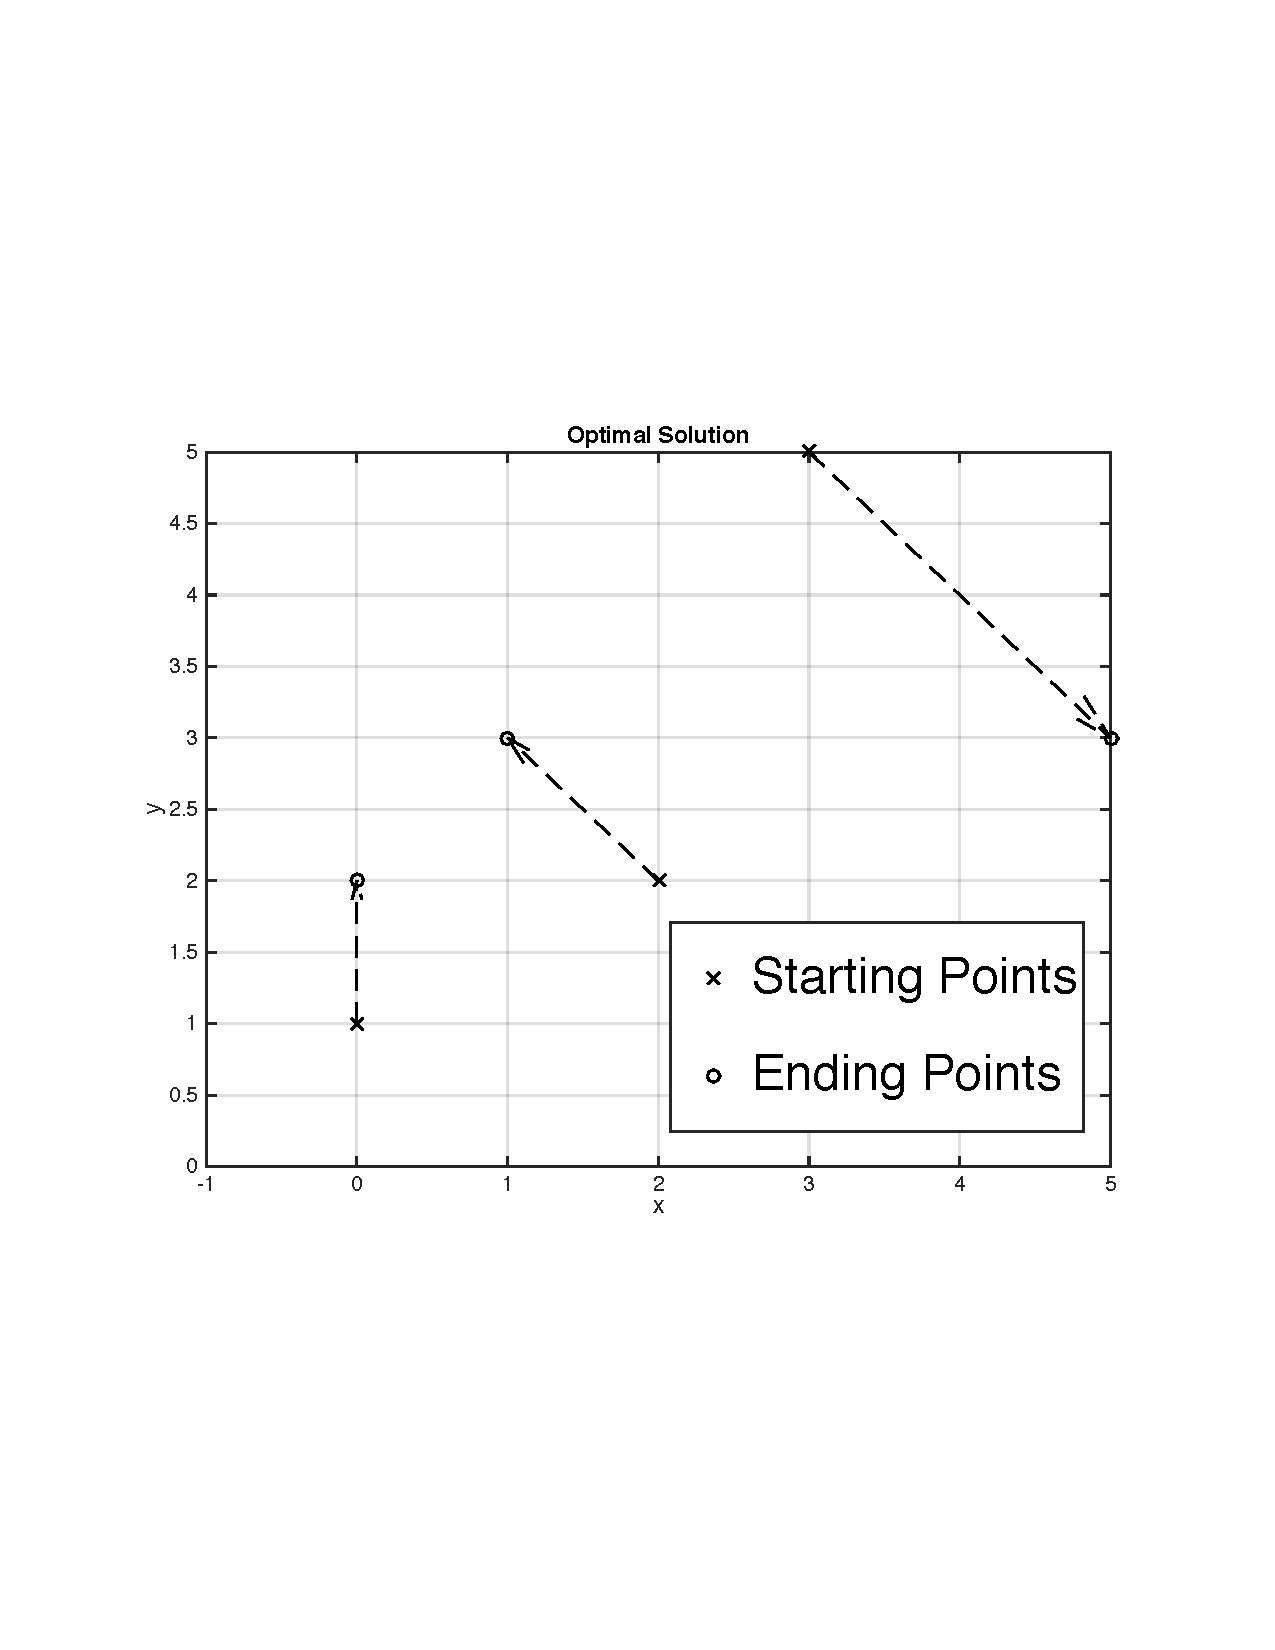
\includegraphics[scale = .4]{1st1DWD.pdf}
  \caption{Discrete Points, WD $\approx$ 1.7475}
  \label{fig: 1Ddiscreet}
\end{subfigure}%
\begin{subfigure}{.5\textwidth}
  \centering
  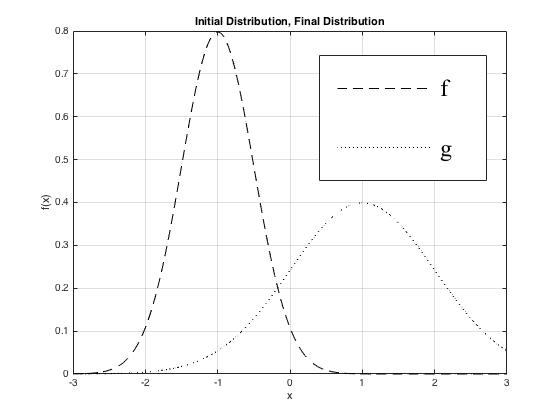
\includegraphics[scale = .4]{1DWDNormal.jpg}
  \caption{Continuous Functions, WD $\approx$ 2.06}
  \label{fig: 1DContinuous}
\end{subfigure}
\caption{Computations of WD in one dimension}
\label{fig:1DWDCalculations}
\end{figure}

\section{Two Dimensional Case}
\label{sec: TwoD}

In two or more dimensions, there is no closed form expression for the Wasserstein distance. One prominent exception is in the case of two Gaussians. If 
\begin{equation}
x \sim \mathcal{N}(\mu_x, \Sigma_x) \text{   and   } y \sim \mathcal{N}(\mu_y, \Sigma_y), 
\end{equation}
and $f, g$ denote the PDFs of $x, y$ respectively, then \cite{Downson}  shows 
\begin{equation}
W_2(f, g) = |\mu_x - \mu_y| +\text{tr}(\Sigma_x + \Sigma_y - 2\sqrt{\Sigma_x\Sigma_y}).
\end{equation}

\noindent In this section a method to approximate the Wasserstein distance between discrete or continuous distributions in $\mathbb{R}^2$ is presented. Consider a physical domain with points $x_{i}, 1 \leq i \leq n \times m$, where $n, m$ are the number of points in the $x, y$ dimensions respectively. Form the matrix $X$ such that $(X)_{j, k}$ is the amount transported from $x_j$ under $f$ to $x_k$ under $g$. Form the matrix $(C)_{j, k} = |x_j - x_k|$ as the distance between points $x_j$ and $x_k.$  With this framework, computing the WD is then equivalent to solving 
\begin{equation}
\begin{aligned}
& {\text{minimize}}
& \sum_{ij}X_{ij}C_{ij} \\
& \text{subject to}
& X\textbf{1} = (a_1, \dotsc, a_m)^{T} \\ 
& & \textbf{1}^{T}X = (b_1, \dotsc, b_n)\\
& & (X)_{ij} \geq 0,
\end{aligned}
\label{eq: dual}
\end{equation}
where \textbf{1} indicates a vector of ones of appropriate length. Because of the linearity of the objective function, (\ref{eq: dual}) can be solved with the simplex method. In Figures \ref{fig: 2Ddiscreet} and \ref{fig: 2DContinuous}, the WD between discreet functions and continuous functions, respectively, in two dimensions is computed.
 
 \begin{figure}[H]
\centering
\begin{subfigure}{.45\textwidth}
  \centering
  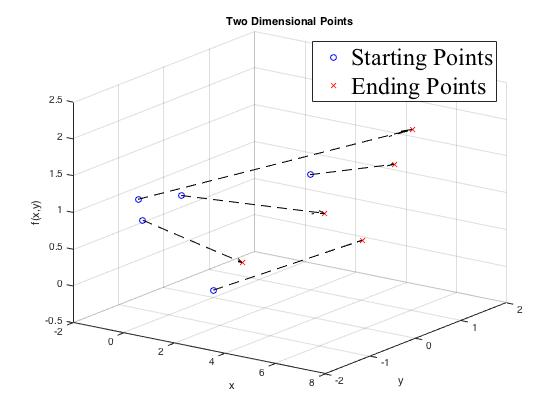
\includegraphics[scale = .4]{2DPoints.jpg}
  \caption{Discrete Points, WD $\approx$ 5.69}
  \label{fig: 2Ddiscreet}
\end{subfigure}%
\begin{subfigure}{.45\textwidth}
  \centering
  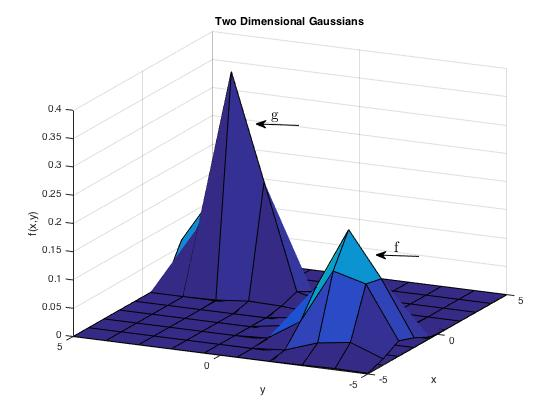
\includegraphics[scale = .4]{2DGaussians.jpg}
  \caption{Continuous Functions, WD $\approx$ 7.12}
  \label{fig: 2DContinuous}
\end{subfigure}
\caption{Computations of WD in two dimensions}
\label{fig:1DWDCalculations}
\end{figure}
\noindent \textbf{Remark:} Although the continuous examples given were normal distributions, the WD can be computed between any two continuous functions. 


 
 


\section{Application to Biological Systems}
\label{sec: BioSystems}
This section applies the tools from previous sections to quantify the differences between biological models that use particles to study larger phenomenon (``micro" models), such as the growth of cancer, and those that study such phenomenon on a macroscopic scope. This question is of critical importance to researchers, since the micro-level models are computationally cheaper and thus providing measures of their accuracy can be very useful. 

\subsection{One Dimensional Case}
For illustration, we begin by examining the growth of cancer cells. To model such a phenomenon on a macroscopic level, we study the model
\begin{equation}
\frac{\partial \rho}{\partial t}  = \frac{\sigma^2}{2}\frac{\partial^2 \rho}{\partial^2 x} + \rho(1-\rho),
\label{eq: MacroModel}
\end{equation}
where $\sigma$ is a scalar and $\rho(x,t)$ denotes the density of cancer cell at time $t$ and a location $x$. For the micro-model, we consider the equation
\begin{equation}
dX_t = \sigma dB_t,
\label{eq: MicroModel}
\end{equation}
where $B_t$ denotes a standard Brownian process, with $B(0) = 0$. For $\Delta t > 0$, we have
\begin{equation}
\int_0^{\Delta t} \ dX_t = \sigma \int_{0}^{\Delta t} \ dB_t \implies x_{\Delta t} - x_0 = \sigma \textbf{Z}
\end{equation}
where $\textbf{Z} \sim \mathcal{N}(0, \Delta t)$. Using properties of variance, 
\begin{equation}
x_{\Delta t} = x_0 + \sigma \sqrt{\Delta t}\textbf{W}
\label{eq: BrownianEQ}
\end{equation} 
where $\textbf{W} \sim \mathcal{N}(0, 1)$. To compute $Micro_{\rho}$, $N \in \mathbb{Z}^+$ i.i.d. realizations of (\ref{eq: BrownianEQ}) are computed, from which a histogram ($Micro_{\rho}$) is created over the physical domain.  In Figures \ref{fig: rhoInitial} and \ref{fig: rhoFinal} we plot $Macro_{\rho}, Micro_{\rho}$ at the initial and final times, respectively.
\begin{figure}[H]
\centering
\begin{subfigure}{.5\textwidth}
  \centering
  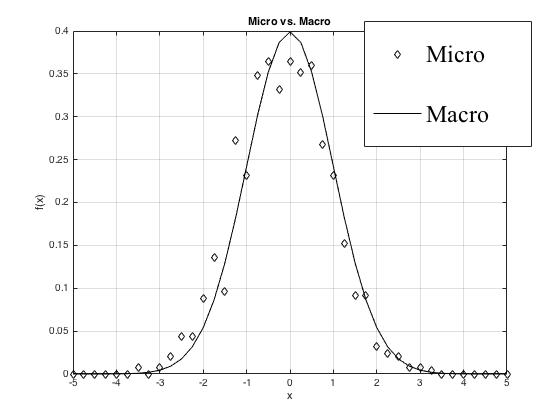
\includegraphics[width=.9\linewidth]{InitialDistributions.jpg}
  \caption{Solutions at initial time}
  \label{fig: rhoInitial}
\end{subfigure}%
\begin{subfigure}{.5\textwidth}
  \centering
  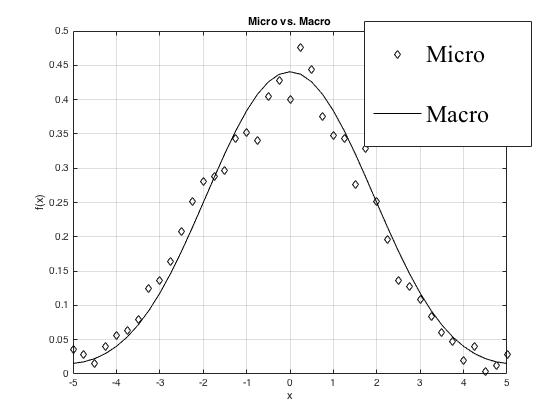
\includegraphics[width=.9\linewidth]{FinalDistribution.jpg}
  \caption{Solutions at final time}
  \label{fig: rhoFinal}
\end{subfigure}
\caption{$N = 10^3, \ T_{final} = 1, \ \Delta t =.01.$}
\label{fig:test}
\end{figure}

\noindent Using a standard normal PDF as the initial condition for $Macro_{\rho}$, and $\Delta x = .05$, we see in Figures \ref{fig:FittingError} and \ref{fig: FittingLogError} the decay of WD and log(WD) against number of particles, respectively. Figure \ref{fig: WDVsX} shows that WD decays linearly a $\Delta x$ decreases.  All WD reported are at $T_{final} = 1, \ \Delta t = .01.$

\begin{figure}
\begin{subfigure}{.5\linewidth}
\centering
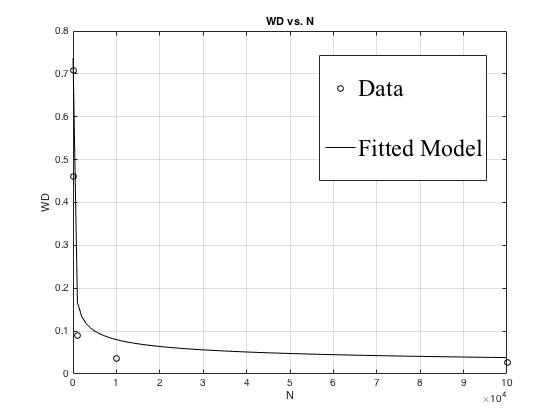
\includegraphics[scale = .4]{WDVSN1D.jpg}
\caption{Fitting WD to N}
\label{fig:FittingError}
\end{subfigure}%
\begin{subfigure}{.5\linewidth}
\centering
\includegraphics[scale = .4]{LogWDVSN1D.jpg}
\caption{Fitting Log(WD) to Log(N)}
\label{fig: FittingLogError}
\end{subfigure}\\[1ex]
\begin{subfigure}{\linewidth}
\centering
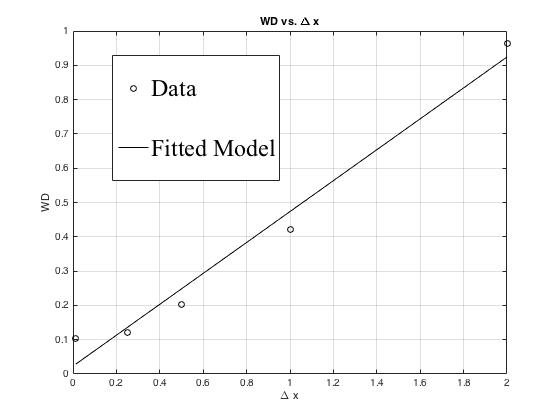
\includegraphics[scale = .4]{WDVSDX.jpg}
\caption{Fitting WD to $\Delta x$}
\label{fig: WDVsX}
\end{subfigure}
\caption{One Dimensional WD Computations}
\label{fig:test}
\end{figure}


\noindent We conclude from Figure \ref{fig:FittingError}  that the error between Macro$_\rho$ and Micro$_\rho$ follows the relationship 
\begin{equation*}
\Big|W_2\Big(Macro_\rho, Micro_\rho\Big)\Big| \approx C\Big({\frac{1}{N}}\Big)^{\alpha},
\end{equation*}
 where $C \approx 3.33, \ \alpha \approx 0.44 $. When computing the fit $log(WD) = a\times log(N) + b$, we find $a \approx -.41,  b \approx .53$. We thus conjecture that the Wasserstein distance between Micro$_\rho$ and Macro$_\rho$ decays at a rate of $1/\sqrt{N}$.
\begin{theorem}
$\Big|W_2\Big(Macro_\rho, Micro_\rho\Big)\Big| \approx C\sqrt{\frac{1}{N}}$, for some $C \in \mathbb{R}$.
\end{theorem}
\begin{proof}
Denote Macro$_\rho$ by $\rho_{mi}$, Micro$_\rho$ by $\rho_{ma}$. Then, for some $\phi \in C_b(\mathbb{R})$
\begin{equation*}
\langle \rho_{mi}, \phi \rangle = \int_{\mathbb{R}} \rho_{mi} \phi(x) \ dx = \frac{1}{N}\sum_x \phi(x_i(t)).
\end{equation*}
By the Law of Large Numbers, 
\begin{equation*}
\frac{1}{N}\sum_x \phi(x_i(t)) \xrightarrow{N \rightarrow \infty} \int_{\mathbb{R}} \phi(x)\rho_{mi}(x) \ dx + \frac{1}{\sqrt{N}}\text{std}(\phi(x))
\end{equation*}
where $\text{std}(\phi(x))$ denotes the standard deviation of $\phi$.
\end{proof}

Figures \ref{fig: MicroVel} and \ref{fig: MacroVel} plot the respective velocities of $Micro_{\rho}, Macro_{\rho}$. To find the velocity between functions $f_1, f_2$ at time $t_j$, we set a value of $c = .1$, then find $x_{j+1} = f_{2}^{-1}(c),  x_{j} = f_{1}^{-1}(c)$. Then, the velocity at time $j$ is $v(j) = \frac{x_{j+1}- x_{j}}{\Delta t}$. Clearly, the velocity of $Micro_{\rho} \approx 1.38 \times 10^2$ is a random variable, while the velocity of $Macro_{\rho}\approx 1.5 \times 10^2$ is deterministic. 

\begin{figure}
\centering
\begin{subfigure}{.5\textwidth}
  \centering
  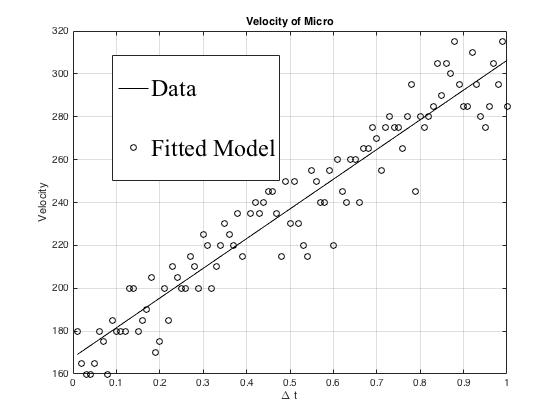
\includegraphics[width=.9\linewidth]{1DMicroVelocity.jpg}
  \caption{Fitting Micro$_{\rho}$ velocity}
  \label{fig: MicroVel}
\end{subfigure}%
\begin{subfigure}{.5\textwidth}
  \centering
  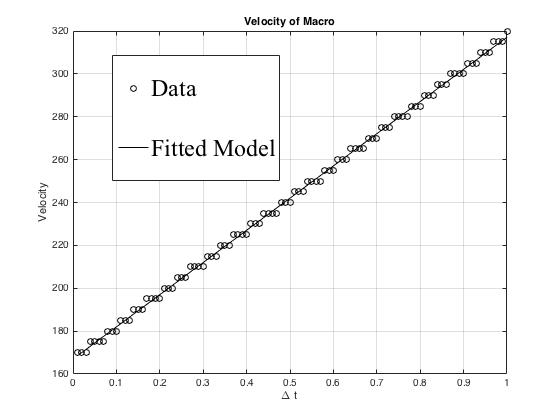
\includegraphics[width=.9\linewidth]{1DMacroVelocity.jpg}
  \caption{Fitting Macro$_{\rho}$ velocity}
  \label{fig: MacroVel}
\end{subfigure}
\caption{Velocities, $T_{final} = 1, \Delta t = .01, N = 10^4, \sigma = \sqrt{2}.$}
\label{fig:test}
\end{figure}

We now investigate how the ratio $\frac{N}{\Delta x}$ impacts the WD. We consider the cases when $(N, \ \Delta x) = (10, 1), \ (10^2, .5), \ (10^3, .125), \ (10^4, .0625).$ For each case, $1,000$ i.i.id realizations of (\ref{eq: MicroModel}) are run. The WD between $Macro_{\rho}$ and $Micro_{\rho}$ at $T_{final = 1},\ \Delta t = .01$ is computed, and then the max of these WD values is computed. We plot the corresponding max WD and pairings of $(N, \ \Delta x)$ in Figures \ref{fig: FittingWDNDX} and \ref{fig: FittingLogWDNDX}.

\begin{figure}
\centering
\begin{subfigure}{.5\textwidth}
  \centering
  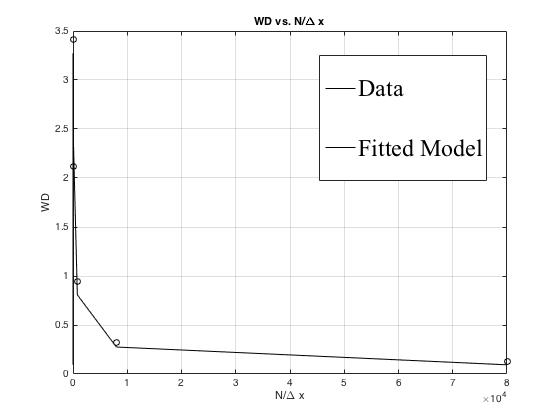
\includegraphics[width=.9\linewidth]{WDVSNDX.jpg}
  \caption{Fitting WD to $\frac{N}{\Delta x}$}
  \label{fig: FittingWDNDX}
\end{subfigure}%
\begin{subfigure}{.5\textwidth}
  \centering
  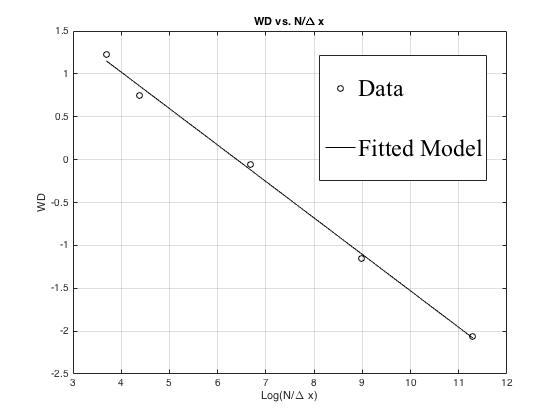
\includegraphics[width=.9\linewidth]{LogWDVSNDX.jpg}
  \caption{Fitting Log(WD) to $Log(\frac{N}{\Delta x})$}
  \label{fig: FittingLogWDNDX}
\end{subfigure}
\caption{One Dimensional WD Computations}
\label{fig:test}
\end{figure}
 




\subsection{Two Dimensional Case}

In two dimensions, the equation for the macro model becomes 
\begin{equation}
\frac{\partial \rho}{\partial t} = D\Big(\frac{\partial^2 \rho}{\partial^2 x} + \frac{\partial^2 \rho}{\partial^2 y}\Big) + \rho(1-\rho),
\label{eq: Macro2D}
\end{equation}
where $\rho(t,x,y)$ denotes the density of cancer cell at time $t$ at location $(x,y).$ Similarly, (\ref{eq: BrownianEQ}) becomes 
\begin{equation}
dX_t = \sigma dB_t,
\label{eq: MicroModel2}
\end{equation}
where $B_t$ denotes a standard Brownian motion in 2 dimensions, with $B(0) = (0,0)$.  Figures \ref{fig:Fitting2DMicroVelocity} and \ref{fig: Fitting2DMacroVelocity}
plot the respective velocities of $Micro_{\rho}, Macro_{\rho}$.  Clearly, the velocity of $Micro_{\rho} \approx $ is a random variable, while the velocity of $Macro_{\rho}\approx 1.5 \times 10^2$ is deterministic. 


\begin{figure}[H]
\centering
\begin{subfigure}{.5\textwidth}
  \centering
  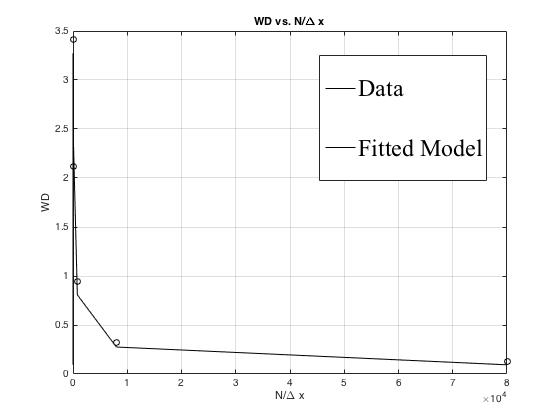
\includegraphics[width=.9\linewidth]{WDVSNDX.jpg}
  \caption{WRONG IMAGE HERE}
  \label{fig:Fitting2DMicroVelocity}
\end{subfigure}%
\begin{subfigure}{.5\textwidth}
  \centering
  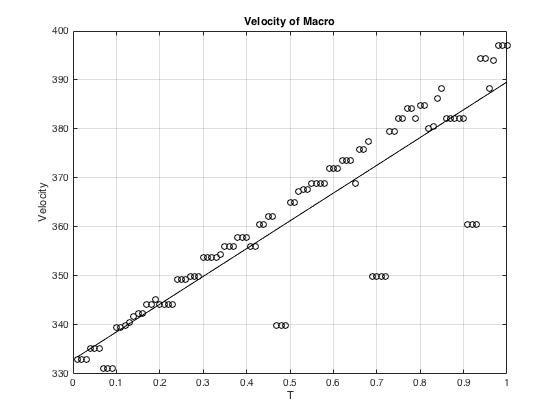
\includegraphics[width=.9\linewidth]{2DMacroVelocity.jpg}
  \caption{Fitting Log(WD) to $Log(\frac{N}{\Delta x})$}
  \label{fig: Fitting2DMacroVelocity}
\end{subfigure}
\caption{2D Velocities, $T_{final} = 1, \Delta t = .01, N = 10^3, \sigma = \sqrt{2}.$}
\label{fig:test}
\end{figure}



\section{Conclusion}
\label{sec: Conclusion}

\section{Definition: More for My Use}
\begin{itemize}
\item Let $X$ be a set. An algebra on $X$ is a collection $\Sigma \subseteq 2^X$ that is closed under finite set operations (complement, union, and intersection). A 
 $\sigma-$algebra on $X$ is a collection $\Sigma \subseteq 2^X$ that is closed under countably many such operations. The intersection of a collection of $\sigma-$algebras is a $\sigma-$algebra. 
 \item A \textbf{Borel set} in a topological space $(X, \mathscr{T})$ is a set that can be made from open sets $U \in \mathscr{T}$ by countable union, countable intersection, or relative complement. The collection of all Borel sets on $X$ forms a $\sigma-$algebra, known as the Borel $\sigma-$algebra, and is denoted by $\mathcal{B}(X)$.
 \item Let $X, Y$ be two topological spaces. A function $f: X \rightarrow Y$ is called a Borel map if 1) $f^{-1}(A)$, A open, is a Borel subset, 2) $f^{-1}(B)$, B closed, is a Borel subset, and 3) $f^{-1}(C)$, C Borel, is a Borel subset.
 \item Given a measurable space (X, $\Sigma$) and a measure $\mu$ on that space, a set $A \subset X$ in $\Sigma$ is called an \textbf{atom} if $\mu(A) > 0$ and for any measurable subset $B \subset A$ with $\mu(B) < \mu(A)$, the set B has measure zero. A measure that has no atoms is called \textbf{non-atomic}.
\end{itemize}

Informal sources:
\begin{itemize}
\item (1) http://www.math.umd.edu/~yanir/OT/AmbrosioGigliDec2011.pdf
\item (2) http://www.math.tohoku.ac.jp/~aida/workshop/H23-Daisympo/kuwada.pdf
\end{itemize}
\begin{thebibliography}{9}% maximum number of references (for label width)
\bibitem{CVillani}
Villani, C., Optimal transport, old and new, June 13, 2008, http://cedricvillani.org/wp-content/uploads/2012/08/preprint-1.pdf 

\bibitem {AN}
Ambrosio, L., Gigli, N. A user's guide to optimal transport.  \url{http://www.math.umd.edu/~yanir/OT/AmbrosioGigliDec2011.pdf}.

\bibitem{Downson}
Dowson, D.C., B.V Landau, The Frechet Distance between Multivariate Normal Distributions, J. Multivariate Analysis 12, 450-455 (1982). 

\bibitem{P}  
Prokhorov, Yu. V., Convergence of random processes and limit theorems in probability theory. (Russian) Teor. Veroyatnost. i Primenen. 1 (1956), 177-238.


\end{thebibliography}

\end{document}
